\section{Istruzioni per l'utilizzo}

\subsection{Primo avvio}
\subsubsection{Selezione del percorso dove sincronizzare}
\label{sec:selezionepath}
Al primo avvio, verrà chiesto di scegliere una cartella dove verranno salvati i file presenti nel server e dove l'utente inserirà i nuovi file che vorrà sincronizzare.
L'utente è obbligato a dover scegliere una cartella, in caso chiudesse la finestra senza aver selezionato una cartella valida, l'applicazione si chiuderà.
\begin{figure}[H]
    \centering
    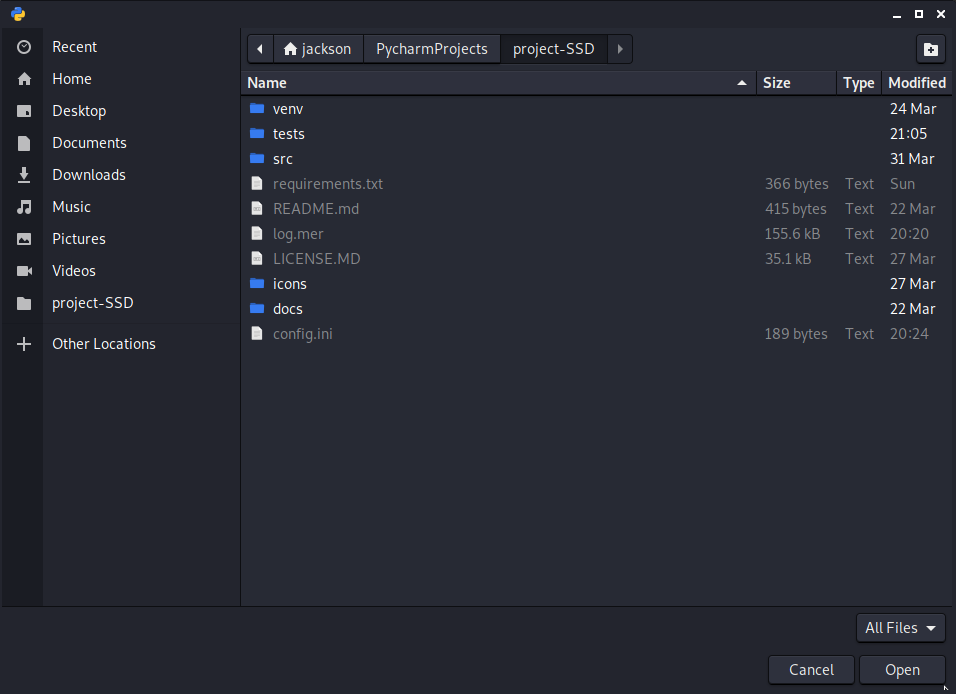
\includegraphics[scale = 0.50]{components/img/selezione-path.png}
    \caption{Selezione del percorso dove sincronizzare}
    \label{fig:Selezione del percorso dove sincronizzare}
\end{figure}


\subsubsection{Autenticazione}
\label{sec:autenticazione}
Successivamente verrà mostrata una form di login, nella quale bisognerà inserire nome utente e password del proprio account \gloman{Zextras Drive} (Fig. \ref{fig:Vista del login}).
Se il login è completato con successo, si avvierà il \gloman{software}, altrimenti verrà visualizzato un messaggio di errore e chiesto di reinserire le credenziali (Fig. \ref{fig:errore login}). \newline
Negli avvii successivi, il login verrà effettuato automaticamente, a meno che non sia stato effettuato il logout (\S{}\ref{sec:profilo}) o la password dell'account sia stata cambiata.
\begin{figure}[H]
    \centering
    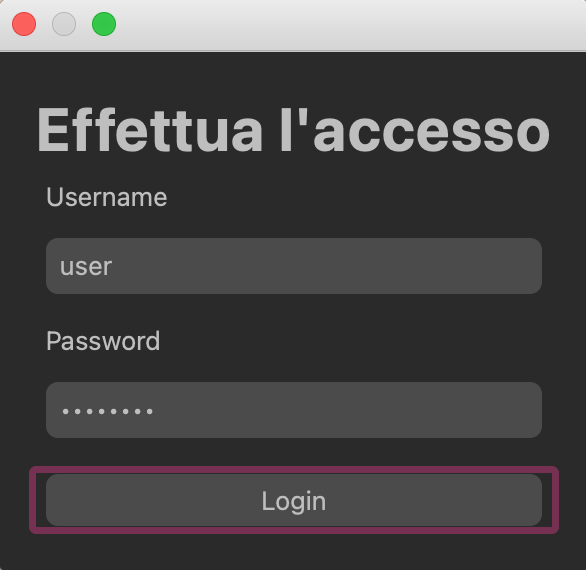
\includegraphics[scale = 0.50]{components/img/login.png}
    \caption{Login}
    \label{fig:Vista del login}
\end{figure}
\begin{figure}[H]
    \centering
    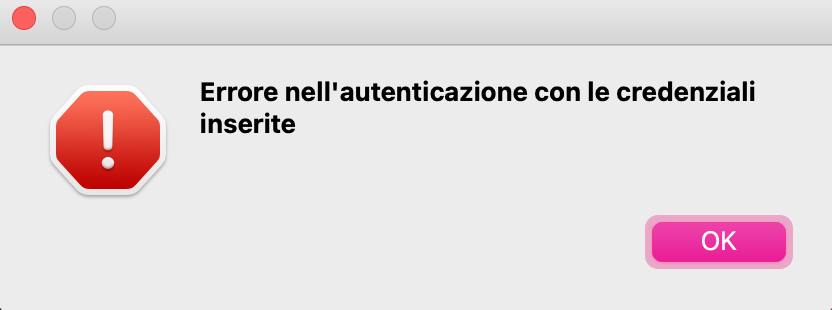
\includegraphics[scale = 0.50]{components/img/err-login.png}
    \caption{Errore di autenticazione}
    \label{fig:errore login}
\end{figure}


\subsection{Finestra principale}
\label{sec:principale}
\begin{figure}[H]
    \centering
    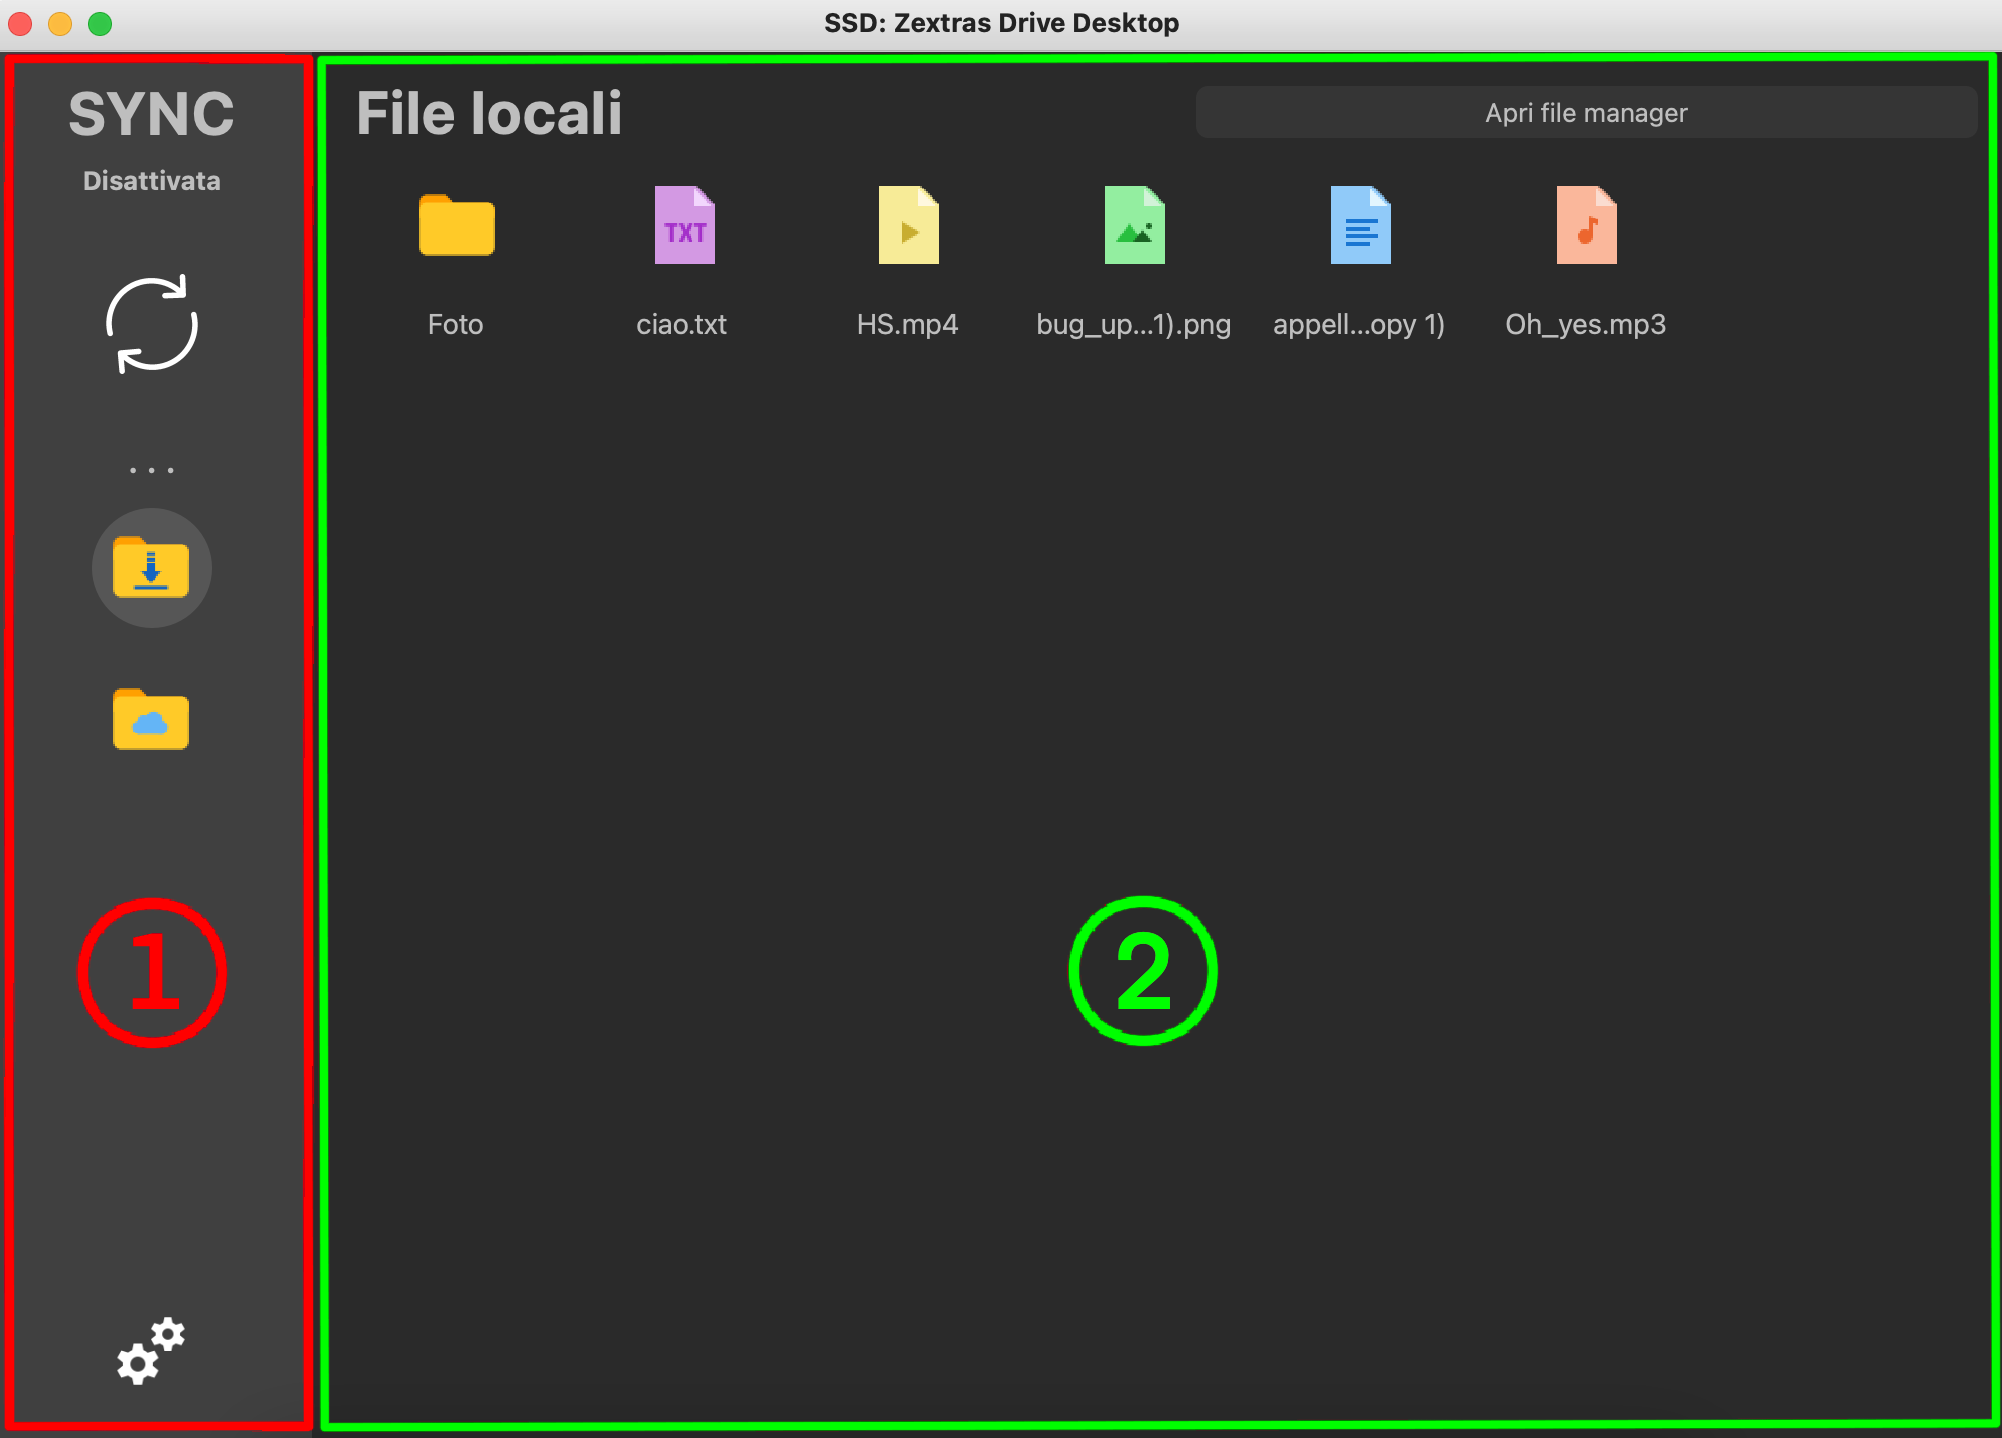
\includegraphics[scale = 0.7]{components/img/Principale.png}
    \caption{Vista schermata principale}
    \label{fig:principale}
\end{figure}
Una volta avviato il software si aprirà una finestra,  mostrata in Fig. \ref{fig:principale}, nella quale verranno visualizzati:
\begin{enumerate}
\item Menù laterale (\S{}\ref{sec:menu});\
\item Finestra principale, che cambia in base al pulsante selezionato nel menù.\
\end{enumerate}


\subsubsection{Menù laterale}
\label{sec:menu}
Il menù laterale è posizionato a sinistra della vista e presenta quattro pulsanti:
\begin{itemize}
\item \textbf{Pulsante di sincronizzazione}: attiva e disattiva la sincronizzazione della cartella locale con il server; \
\end{itemize}
\begin{figure}[H]
\centering
\begin{minipage}[b]{0.45\linewidth}
\centering

\includegraphics[scale=0.5]{components/img/SyncA.png}
\caption{Sincronizzazione attivata}
\label{fig:PsyncA}
\end{minipage}
\quad
\begin{minipage}[b]{0.45\linewidth}
\centering
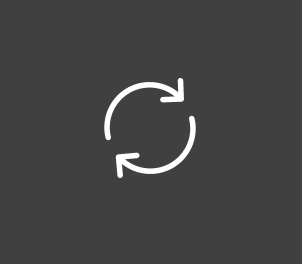
\includegraphics[scale=0.5]{components/img/SyncD.png}
\caption{Sincronizzazione disattivata}
\label{fig:PsyncD}
\end{minipage}
\end{figure}
\begin{itemize}
\item \textbf{Pulsante file sincronizzati}: mostra la cartella locale sincronizzata (\S{}\ref{sec:fileLocali}); \
\end{itemize}
\begin{figure}[H]
    \centering
    
\includegraphics[scale = 1]{components/img/pulsanteFileS.png}
    \caption{Pulsante file sincronizzati}
    \label{fig:PfileSync}
\end{figure}
\begin{itemize}
\item \textbf{Pulsante file remoti}: mostra i file presenti nel server (\S{}\ref{sec:fileRemoti}); \
\end{itemize}
\begin{figure}[H]
    \centering
    
\includegraphics[scale = 1]{components/img/pulsanteFileR.png}
    \caption{Pulsante file remoti}
    \label{fig:PfileRem}
\end{figure}
\begin{itemize}
\item \textbf{Pulsante delle impostazioni}: mostra le impostazioni del software (\S{}\ref{sec:impostazioni}). \
\end{itemize}
\begin{figure}[H]
    \centering
    
\includegraphics[scale = 1]{components/img/pulsanteImpostazioni.png}
    \caption{Pulsante impostazioni}
    \label{fig:PImp}
\end{figure}

\subsection{Operazioni comuni}
In questa sezione vengono elencati i passaggi necessari per eseguire le operazioni più comuni previste dal programma.
\subsubsection{Scaricare un file dal server}
\begin{itemize}
\item Attivare la sincronizzazione cliccando il pulsante di sincronizzazione (\ref{fig:PsyncD});
\item Cliccare sul pulsante per visualizzare i file remoti (\ref{fig:PfileRem});
\item Navigare fino al file desiderato ed eseguire un click destro su di esso, quindi selezionare la voce "aggiungi a sync" dal menu contestuale;
\item Il file verrà sincronizzato allo scadere dell'intervallo di tempo di sincronizzazione selezionato, nel caso si volesse sincronizzare immediatamente il file è necessario cliccare sul pulsante per visualizzare i file sincronizzati (\ref{fig:PfileSync}) e cliccare sul pulsante "sincronizza ora".
\end{itemize}
\subsubsection{Eliminare un file dal server}
\begin{itemize}
\item Attivare la sincronizzazione cliccando il pulsante di sincronizzazione (\ref{fig:PsyncD});
\item Cliccare sul pulsante per visualizzare i file sincronizzati (\ref{fig:PfileSync});
\item Cliccare il pulsante "apri file manager";
\item Eliminare il file desiderato dal file manager;
\item Premere il pulsante "sincronizza ora" per aggiornare il server con i file locali, eliminando quindi il file eliminato in locale dal server.
\end{itemize}
\subsubsection{Rimuovere un file dalla sincronizzazione}
\begin{itemize}
\item Cliccare sul pulsante per visualizzare i file remoti (\ref{fig:PfileRem});
\item Navigare fino al file sincronizzato desiderato ed eseguire un click destro su di esso, quindi selezionare la voce "rimuovi da sync" dal menu contestuale. Il file verrà conservato in locale ma gli aggiornamenti ad esso non verranno più sincronizzati con il server e viceversa.
\end{itemize}


\subsection{Azioni sui file}
\label{sec:fileActions}

\subsubsection{Doppio click su un file}
Eseguendo un doppio click su un file nella vista File locali (\ref{sec:fileLocali}) il file verrà aperto dall'applicazione designata dal sistema.
\subsubsection{Click destro su un file}
Eseguendo un click destro su un file nella vista File remoti (\ref{sec:fileRemoti}) è possibile aggiungere o rimuovere un file dalla lista di sincronizzazione.  
\subsubsection{Doppio click su una cartella}
Eseguendo un doppio click su di una cartella, sia nella vista File locali che in quella File remoti, si scenderà di un livello, visualizzando il contenuto della cartella selezionata.
\subsubsection{Inserire file nella cartella locale}
Per inserire file nella cartella locale è necessario aprire il file manager utilizzando l'apposito pulsante e aggiungere file da esso.
\subsubsection{Refresh del server}
Per aggiornare la lista dei file visualizzati nella vista \ref{sec:fileRemoti} con le ultime modifiche avvenute nel server bisogna premere il pulsante "Refresh".
\subsubsection{Modifica di un file sincronizzato}
La modifica di un file sincronizzato avviene in maniera analoga alla modifica di un qualsiasi file locale, dopo aver effettuato i cambiamenti necessari è sufficiente salvare il documento e questo verrà automaticamente sincronizzato con il server.
\subsubsection{Cancellazione di un file sincronizzato}
L'eliminazione di un file sincronizzato avviene analogamente all'eliminazione di un qualsiasi file locale, dopo aver eliminato il file dalla cartella sincronizzata questa modifica verrà propagata anche nel server.

\subsection{File locali}
\label{sec:fileLocali}
\begin{figure}[H]
    \centering
    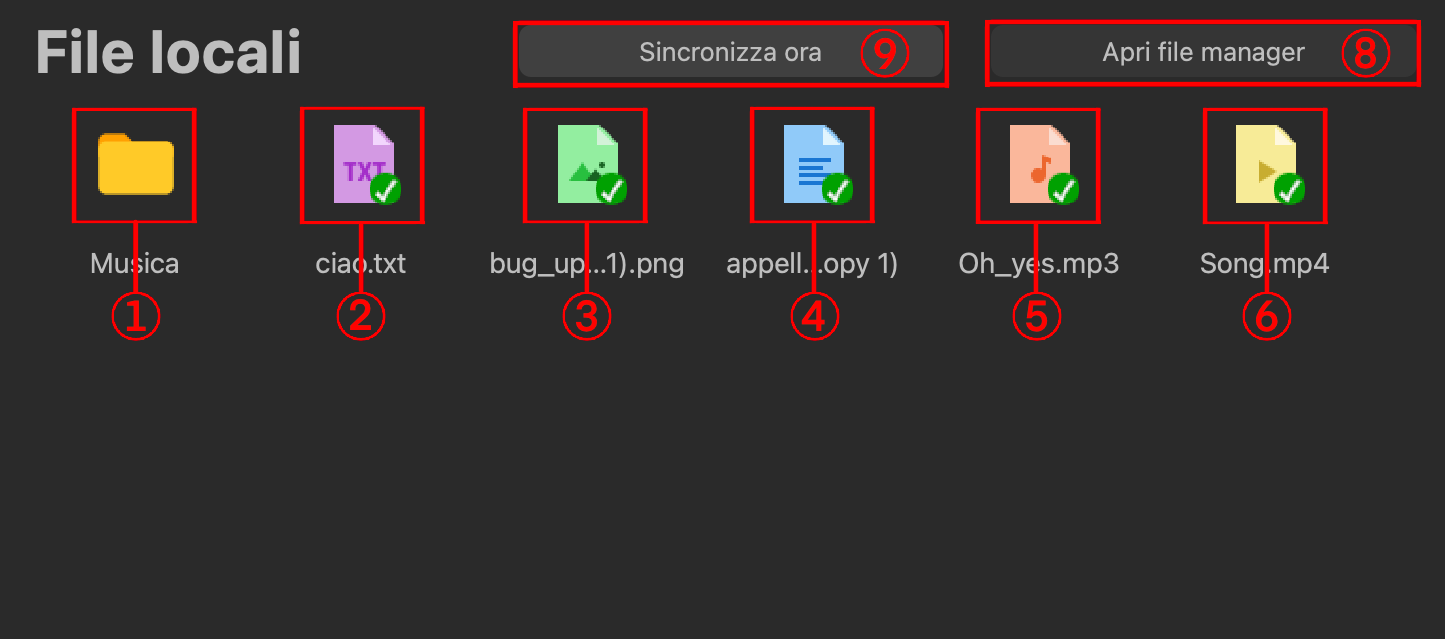
\includegraphics[scale = 0.9]{components/img/fileLocali.png}
    \caption{Vista file locali}
    \label{fig:fileSync}
\end{figure}
La vista si compone di una serie di icone che rappresentano i file o le cartelle presenti nella cartella condivisa. Le icone possono rappresentare:
\begin{itemize}
\item \textbf{Cartella [1]};\
\item \textbf{File di testo [2]};\
\item \textbf{File immagine [3]};\
\item \textbf{File generico [4]};\
\item \textbf{File audio [5]};\
\item \textbf{File video [6]}.\
\end{itemize}
In alto a destra ci sono due pulsanti:
\begin{itemize}
\item \textbf{Sincronizza ora [7]}: permette di forzare la sincronizzazione con il server;\
\item \textbf{Apri file manager [8]}: apre la cartella rappresentata tramite il file manager del computer.\
\end{itemize}


\subsection{File remoti}
\label{sec:fileRemoti}
\begin{figure}[H]
    \centering
    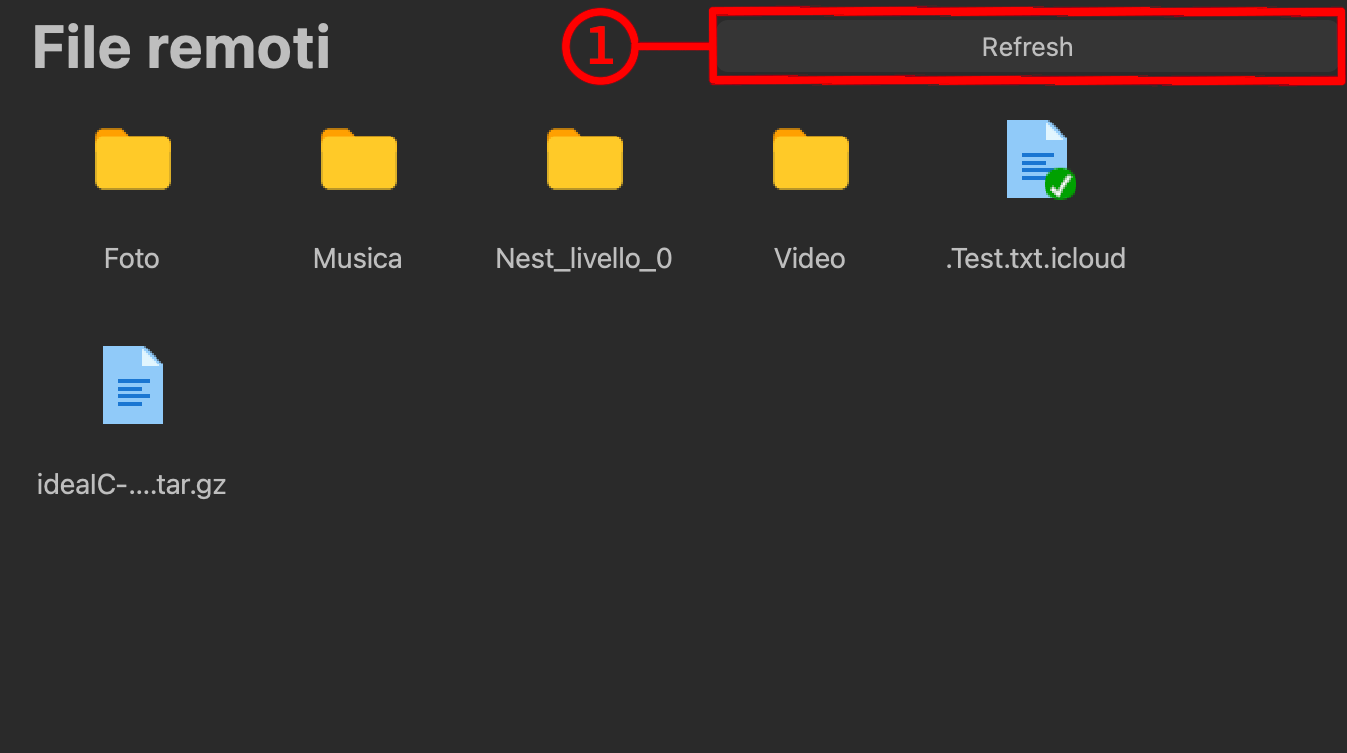
\includegraphics[scale = 0.8]{components/img/fileRem.png}
    \caption{Vista file remoti}
    \label{fig:fileRem}
\end{figure}
La vista si compone di una serie di icone che rappresentano i file o le cartelle presenti nella cartella remota. In alto a destra è presente un pulsante \textbf{[1]} che permette di effettuare il refresh della cartella remota.

\subsubsection{Tooltip}
\label{sec:fileRemotiTooltip}
\begin{figure}[H]
    \centering
    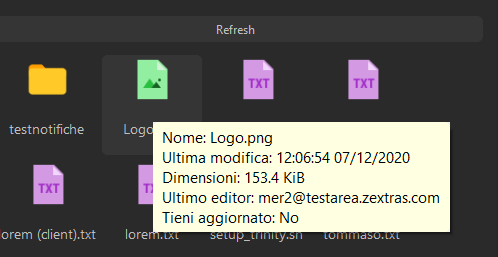
\includegraphics[scale = 0.8]{components/img/fileRem_tooltip.png}
    \caption{Tooltip in file remoti}
    \label{fig:fileRemotiTooltip}
\end{figure}
Per ogni file l'utente può visionare le seguenti informazioni:
\begin{itemize}
    \item \textbf{Nome};
    \item \textbf{Ultima modifica};
    \item \textbf{Dimensioni};
    \item \textbf{Ultimo editor}: Nel caso l'utente abbia condiviso la sua cartella con altri utenti, può vedere chi è stata l'ultima persona ad averlo modificato;
    \item \textbf{Tieni aggiornato}.
\end{itemize}

\subsection{Icone di sincronizzazione}
\label{sec:iconeSync}
Per far sì che l'utente capisca a colpo d'occhio lo stato dei file ci sono tre icone che appariranno a seconda del caso in questione.
\subsubsection{Spunta su sfondo verde}

\begin{figure}[H]
    \centering
    
\includegraphics[scale = 0.8]{components/img/iconIsSync.png}
    \caption{Icona file sincronizzato}
    \label{fig:greenI}
\end{figure}

L'icona rappresentata in figura apparirà sui file presenti nella cartella locale e significa che il file è sincronizzato con il server.
\subsubsection{Frecce su sfondo blu}

\begin{figure}[H]
    \centering
    
\includegraphics[scale = 1.6]{components/img/iconSync.png}
    \caption{Icona file in sincronizzazione}
    \label{fig:bluedownI}
\end{figure}

L'icona rappresentata in figura apparirà sui file presenti nella cartella locale e significa che il file sta venendo sincronizzato con il server.

\subsubsection{Freccia verso il basso su sfondo blu}

\begin{figure}[H]
    \centering
    
\includegraphics[scale = 0.8]{components/img/iconUpdate.png}
    \caption{Icona file segnato da aggiornare}
    \label{fig:greenI}
\end{figure}


L'icona rappresentata in figura apparirà sui file presenti nella cartella remota e significa che quel file verrà aggiornato ogni volta che nel server sono presenti delle modifiche.

\subsection{Notifiche}
L'applicazione può inviare all'utente le seguenti notifiche:
\begin{itemize}
    \item Uno o più file sono stati scaricati;
    \item Uno o più file sono stati aggiornati;
    \item L'applicazione non è in grado di connettersi ad internet;
    \item L'utente ha esaurito la quota disco, quindi i file non possono essere scaricati;
    \item Le credenziali sono state cambiate, l'utente deve aggiornarle all'interno dell'applicazione.
\end{itemize}
Le notifiche che l'utente vedrà più spesso sono quelle relative ai file aggiornati e scaricati.
\begin{figure}[H]
    \centering
    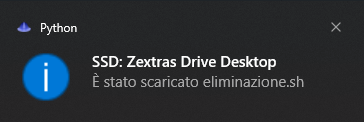
\includegraphics[scale = 0.7]{components/img/notifica_download_new_file.png}
    \caption{Notifica di un nuovo file che è stato scaricato}
    \label{fig:impostazioni}
\end{figure}
\begin{figure}[H]
    \centering
    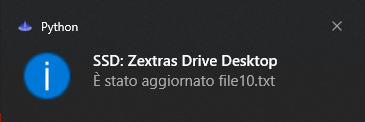
\includegraphics[scale = 0.7]{components/img/notifica_download_update_file.png}
    \caption{Notifica di un file che è stato aggiornato}
    \label{fig:impostazioni}
\end{figure}

\subsection{Impostazioni}
\label{sec:impostazioni}
\begin{figure}[H]
    \centering
    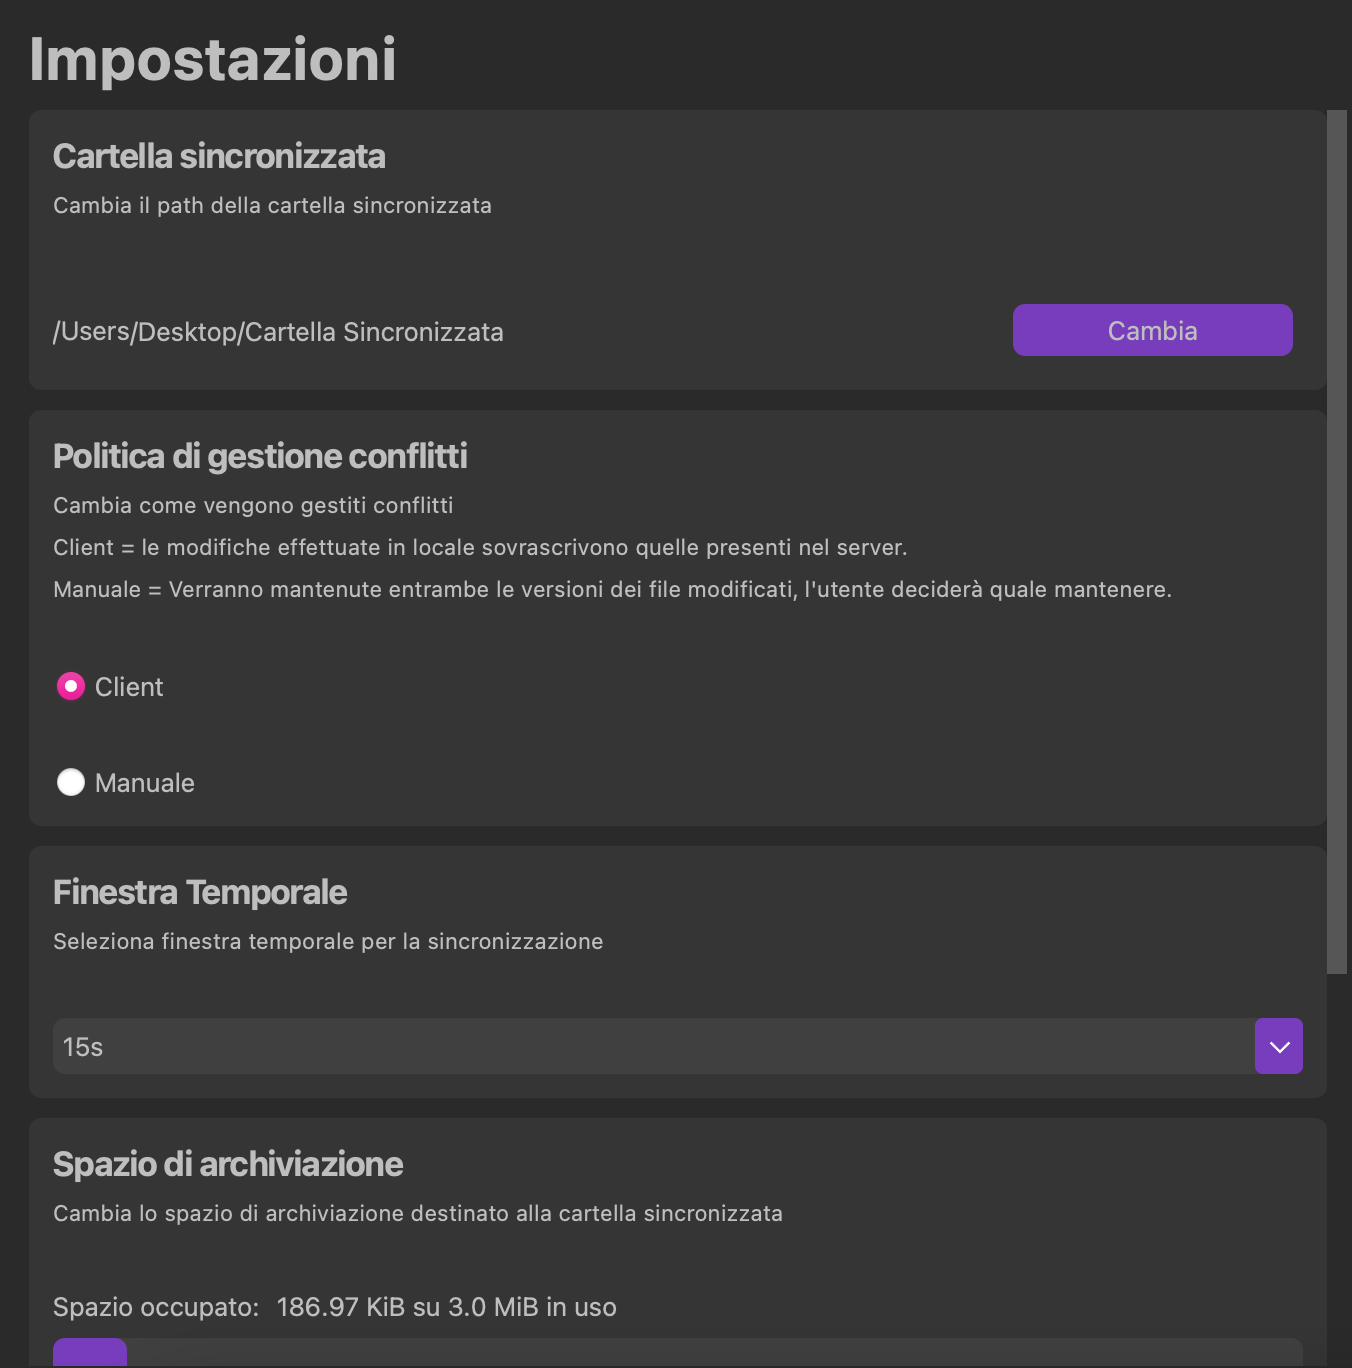
\includegraphics[scale = 0.7]{components/img/vistaImp.png}
    \caption{Vista impostazioni}
    \label{fig:impostazioni}
\end{figure}
La vista mostra una serie di riquadri con i quali è possibile interagire per modificare le impostazioni legate al software. Tramite l'apposita barra posizionata sulla destra è possibile visualizzare l'intera pagina delle impostazioni.

\subsubsection{Modifica path cartella}
\label{sec:cartella}
\begin{figure}[H]
    \centering
    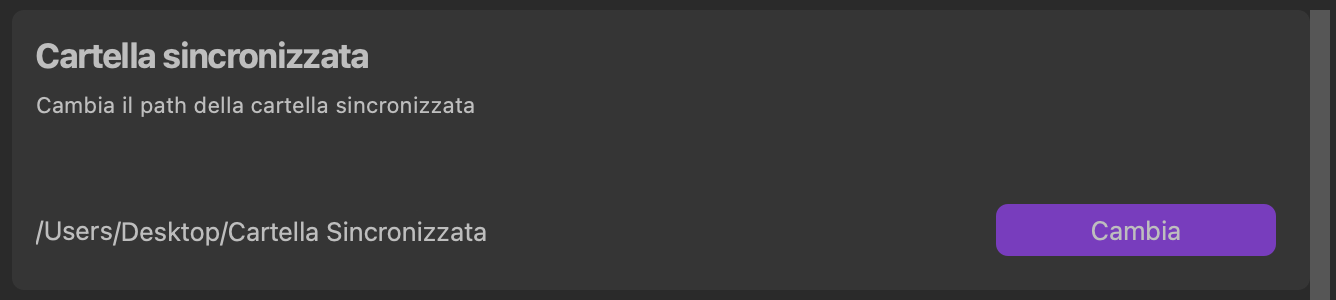
\includegraphics[scale = 1]{components/img/ImpCartella.png}
    \caption{Modifica percorso cartella}
    \label{fig:cartella}
\end{figure}
In questa sezione delle impostazioni è possibile modificare il percorso della cartella sincronizzata. Premendo il pulsante "Cambia" si aprirà una finestra che permetterà di cambiare il percorso (\S{}\ref{sec:selezionepath}).

\subsubsection{Modifica policy}
\label{sec:policy}
\begin{figure}[H]
    \centering
    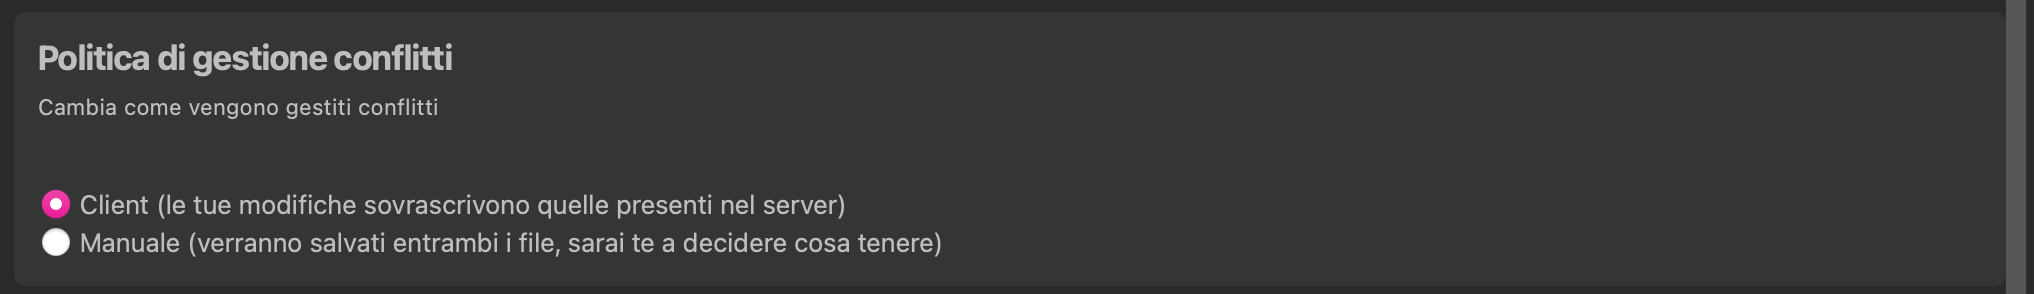
\includegraphics[scale = 0.4]{components/img/ImpPolicy.png}
    \caption{Modifica politica di risoluzione conflitti}
    \label{fig:policy}
\end{figure}
In questa sezione è possibile scegliere la politica di risoluzione dei conflitti. Ci sono due opzioni:
\begin{itemize}
\item\textbf{Client:} selezionando questa opzione le modifiche effettuate in locale andranno a sovrascrivere quelle caricate nel server;\
\item\textbf{Manuale:} selezionando questa opzione, ogni volta che il file in locale differisce dal file presente nel server verranno salvate entrambe le versioni in locale e sarà l'utente a decidere quale mantenere.\
\end{itemize}

\subsubsection{Modifica finestra temporale}
\label{sec:finestra temporale}
\begin{figure}[H]
    \centering
    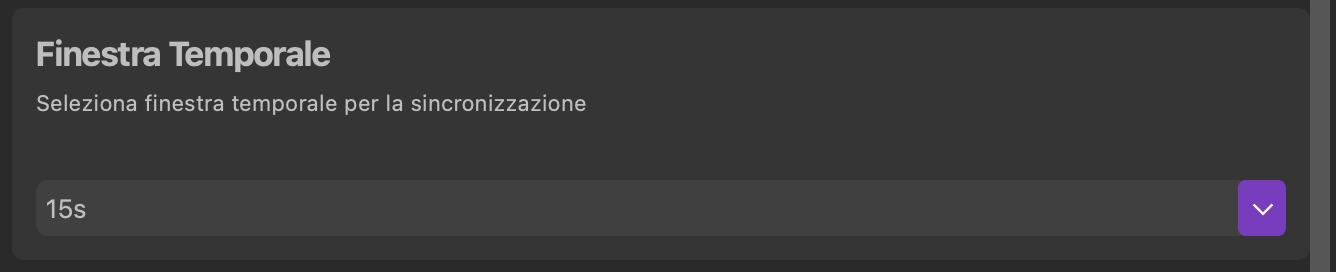
\includegraphics[scale = 0.65]{components/img/ImpFinTempA.png}
    \caption{Modifica finestra temporale}
    \label{fig:finTempA}
\end{figure}
In questa sezione è possibile modificare ogni quanto tempo avviare la sincronizzazione dal server alla cartella condivisa. Cliccando sull'apposita freccia a destra (Fig. \ref{fig:finTempC}) apparirà un elenco di possibili finestre temporali. 
\begin{figure}[H]
    \centering
    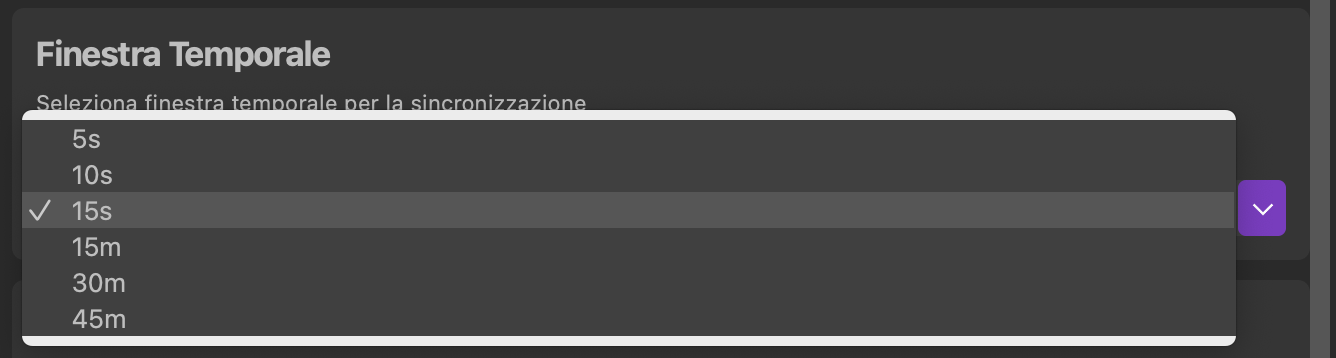
\includegraphics[scale = 0.65]{components/img/ImpFinTempC.png}
    \caption{Vista dopo aver cliccato sulla freccia}
    \label{fig:finTempC}
\end{figure}

\subsubsection{Modifica spazio di archiviazione}
\label{sec:quota}
\begin{figure}[H]
    \centering
    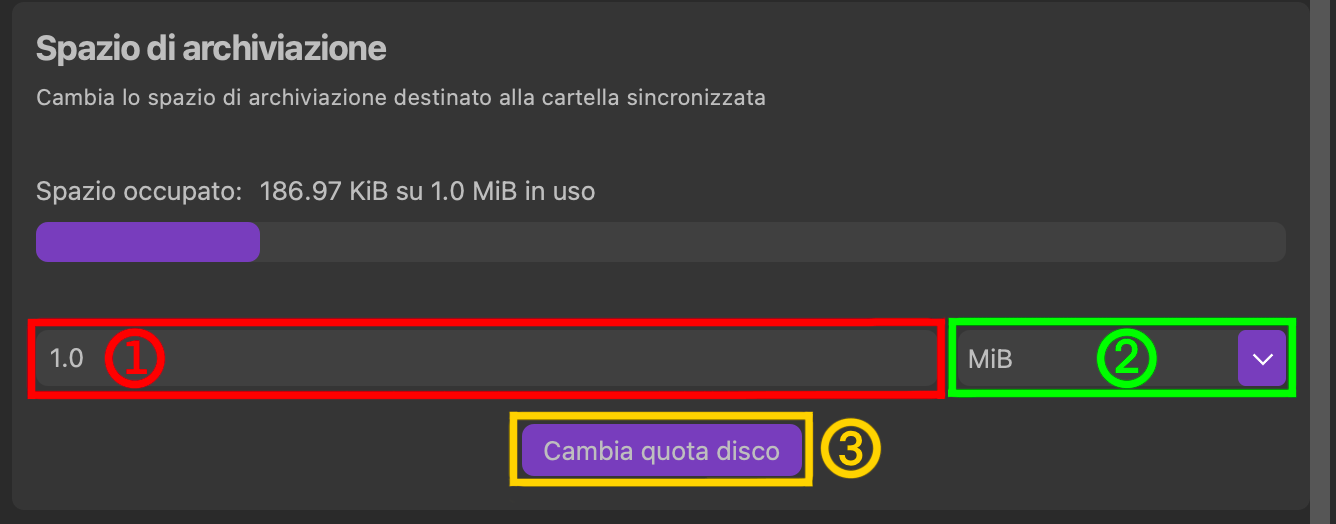
\includegraphics[scale = 0.8]{components/img/ImpQuota.png}
    \caption{Modifica quota disco}
    \label{fig:quota}
\end{figure}
In questa sezione è possibile modificare lo spazio di archiviazione dedicato alla cartella locale. In particolare, seguendo i numeri in Fig. \ref{fig:quota}:
\begin{enumerate}
\item permette di scrivere quanto spazio far occupare alla cartella;\
\item permette di decidere l'estensione del numero scritto (Fig. \ref{fig:quotazoom});\
\item pulsante che modifica lo spazio di archiviazione.\
\end{enumerate}
\begin{figure}[H]
    \centering
    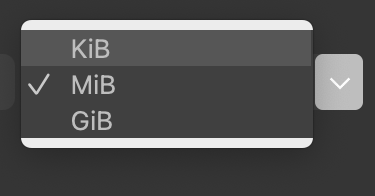
\includegraphics[scale = 1]{components/img/ImpQuota2.png}
    \caption{Vista dopo aver cliccato sulla freccia}
    \label{fig:quotazoom}
\end{figure}


\subsubsection{Profilo}
\label{sec:profilo}
\begin{figure}[H]
    \centering
    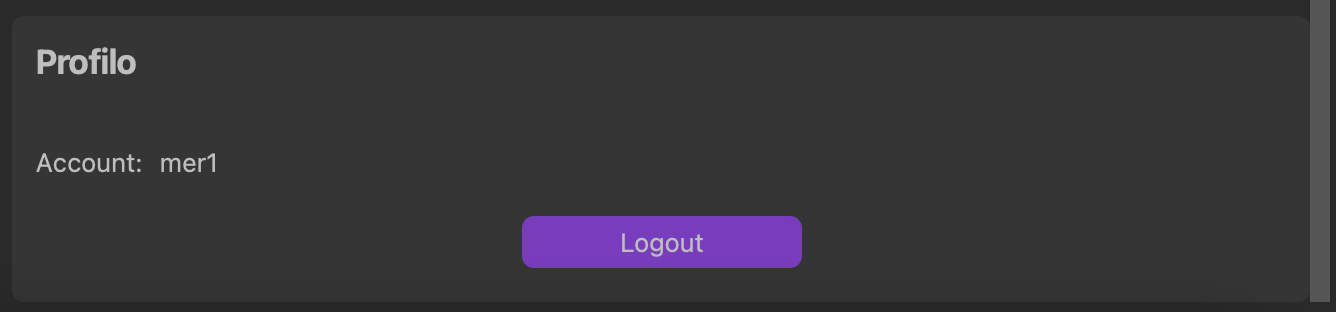
\includegraphics[scale = 0.65]{components/img/ImpLogout.png}
    \caption{Vista logout}
    \label{fig:fileRem}
\end{figure}
In questa sezione è possibile visualizzare il profilo collegato alle credenziali inserite. Inoltre, premendo il pulsante "Logout", è possibile disconnettere il profilo dal software: quest'ultimo si chiuderà e, al prossimo avvio, mostrerà la schermata di login (\S{}\ref{sec:autenticazione})

